\section{Missing Details from the Experiments}\label{app_experiments}


\subsection{Synthetic Settings}\label{app_synthetic}
	We describe the parameter settings used in the synthetic experiments (Figure \ref{fig_model_shift_phasetrans}).
	For all three synthetic experiments, we set the input feature dimension as $p = 200$.
	\squishlist
		\item Task similarity: We use $\rho_1 = 90, \rho_2 = 30$ for sample sizes.
	The noise level is $\sigma = 5$.
	We set $\kappa = 1$ and vary model distance $d$ from $0.01$ to $0.2$.
	The $x$-axis measures the function $\Phi(\beta_1, \beta_2)$ described in Section \ref{sec_similarity}.
	The $y$-axis measures the improvement of prediction loss using MTL compared to STL.
		\item Sample size: We set $\kappa = 1$ and $d = 0.02$ for model distance.
	We use $\rho_2 = 500$ and vary $\rho_1$ from $50$ to $800$ for sample sizes.
		\item Covariate shift: We set $\kappa = 1$ and $d = 0$.
	We set $\rho_2 = 4$ and vary $\rho_1$ from $5$ to $25$ for sample sizes.
	We use the scale parameter $\lambda = 1$ for the curve without covariate shift and $\lambda = 2$ for the curve with covariate shift (cf. Section \ref{sec_covshift}).
	Without loss of generality, we have rescaled the $x$ and $y$ axis for the ease of presentation.
	This can be achieved similarly by rescaling the task data.
	\squishend

\subsection{Image and Text Classification Settings}\label{app_it}

For the text classification experiment, we encode each word using the GLoVe word embeddings.%
\footnote{http://nlp.stanford.edu/data/wordvecs/glove.6B.zip}
We evaluate three model choices.
For multi-layer perception (MLP), we apply an average pooling layer over the word embeddings.
For LSTM and CNN, we add a shared feature representation layer on top of the word embeddings \cite{lei2018simple}.

\textit{Predicting transfer effect via STL results.}
We simplify the setup of this experiment by fixing the sample sizes of every task pair.
For sentiment analysis tasks, the sample size of the source task ranges in $500, 1000, 1500$.
We randomly sample these many data points from the task.
The sample size of the target task is $1000$.
For image classification tasks, the training sample size is $10,000$ for every task.

\textit{Mitigating negative transfer via incremental training.}
For the case of two tasks, we compare the incremental training scheduled described in Algorithm \ref{alg_inc_train}  to a round-robin training schedule baseline.
We add $20\%$ of source task samples for every $T = 2$ epochs.
The total number of epochs is $20$.
We set the threshold $\tau$ as the validation accuracy of the target task using the baseline training schedule.

For the case of six tasks, we extend Algorithm \ref{alg_inc_train} accordingly.
Initially, we use $5\%$ of samples from SST and $50\%$ of samples from the other tasks.
We add $19\%$ of samples from SST and $5\%$ of samples from the other tasks for every $2$ epochs.
We run $20$ epochs in total.

\begin{algorithm}[!t]
	\caption{An incremental training schedule for efficient multi-task learning with two tasks}
	\label{alg_inc_train}
	\begin{algorithmic}[1]
		\Input Two tasks $(X_1, Y_1)$ and $(X_2, Y_2)$.
		\Param A shared module $B$, output layers $W_1, W_2$ as in the hard parameter sharing architecture.
		\Req \# batches $S$, epochs $T$, task $2$'s validation accuracy $\hat{g}(B; W_2)$, a threshold $\tau\in(0,1)$.
		\Output The trained modules $B, W_2$ optimized for task $2$.
		\State Divide $(X_1, Y_1)$ randomly into $S$ batches: $(x^{(1)}, y^{(1)}), \dots, (x^{(S)}, y^{(S)})$.
		\For{$i = 1,\dots, S$}
			\For{$j = 1,\dots, T$}
				\State Update $B, W_1, W_2$ using the training data $\set{x^{(k)}, x^{(k)}}_{k=1}^i$ and  $(X_2, Y_2)$.
			\EndFor
			\State Let $a_i = \hat{g}(B; W_2)$ be the validation accuracy.
			\If{$a_i < a_{i-1}$ or $a_i > \tau$}
				\State \textbf{break}
			\EndIf
		\EndFor
	\end{algorithmic}
\end{algorithm}




\textit{Validating the Theoretical Results.}
We fill in the details of the experimental procedure used for the results in Figure \ref{fig_ablation}.
\squishlist
	\item Task similarity: We select a similar and a dissimilar source task compared to the target task using domain knowledge.
First pair: the customer review dataset (CR) , which predicts whether a review is positive or negative, is more similar to SST (sentiment treebank) than MPQA (question type).
Second pair: SST is more similar to MR since they both concern about positive or negative opinions expressed the text.
TREC is less similar to MR because the task is about question types.
Third pair: MPQA (opinion polarity) is more similar to TREC (question type)
	\item Sample size: We vary the sample size of the source task from $100$ to $3000$.
	\item Covariate shift: We implement the covariance alignment procedure following \cite{WZR20}.
	We fix the sample size of the target task as $1000$.
\squishend

%We validate that MTL performs better when the source task is more similar to the target task.
%We show the result on the sentiment analysis tasks.
%For a target task, we manually select a similar task and a dissimilar task based on prior knowledge.
%Figure \ref{fig_ab_sim} confirms the result.
%Recall that Section \ref{sec_data_size} shows that increasing the data size of the source task does not always improve the performance of MTL for the target task.
%In Figure \ref{fig_ab_data}, we show that for source task MR and target task SST, there is a transition from positive to negative transfer as we increase the data size of the source task.
%Our result provides a fine-grained insight on the covariance alignment algorithm proposed in \cite{WZR20}.
%Recall that the covariance alignment procedure in \cite{WZR20} adds an additional module between the word embedding representation and the shared module.
%When the source task data size is particularly large compared to the target task, we show that applying the covariance alignment algorithm results in more significant gains.
%In Figure \ref{fig_ab_cov}, we observe that the benefit from aligning task covariances becomes more significant for LSTM and MLP as we increase the number of datapoints of the source task.

\textbf{Further results of the covariance alignment procedure.}
Our results in Figure \ref{fig_ab_cov} are averaged over all the task pairs.
In Figure \ref{fig_covariate_app}, we show two task pairs as examples.
In Figure \ref{fig_cov_a}, we observe that for the particular task pair, covariance alignment provides more significant gains when the sample ratio is large.
In Figure \ref{fig_cov_b}, we observe that covariance alignment does not always improve over the baseline multi-task learning model.
One explanation is that MR and SST are similar tasks, hence adding the alignment module is unnecessary.
An interesting question is to understand when adding the alignment module benefits the multi-task learning model.
We leave this question for future work.
%Note: For text classification tasks, the source task training data size ranges from 500 to 1,500 and target task training data size is 1000; For ChestX-ray14,

\begin{figure}[!h]
	\centering
	\begin{subfigure}[b]{0.48\textwidth}
		\centering
		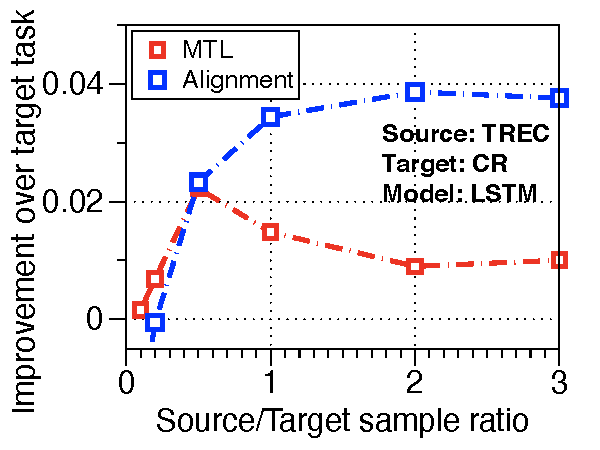
\includegraphics[width=0.7\textwidth]{figures/ratio_alignment_norm_trec_cr_lstm.pdf}
		\caption{Task pair TREC and CR}
		\label{fig_cov_a}
	\end{subfigure}\hfill
		\begin{subfigure}[b]{0.48\textwidth}
		\centering
		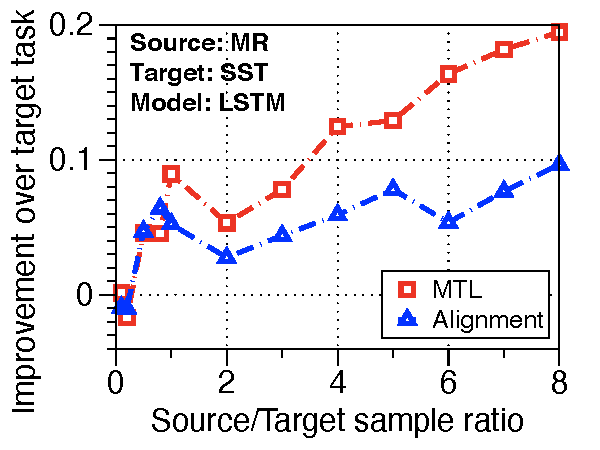
\includegraphics[width=0.7\textwidth]{figures/ratio_alignment_mr_sst_lstm.pdf}
		\caption{Task pair MR and SST}
			\label{fig_cov_b}
	\end{subfigure}
	\caption{(a) For the task pair TREC and CR, adding the covariance alignment procedure provides more improvement when the source/target sample ratio is large.
	(b) For the task pair MR and SST, adding the covariance alignment procedure hurts performance.
	One explanation is that MR and SST are similar tasks, hence adding the alignment module is unnecessary.}
	\label{fig_covariate_app}
\end{figure}
